\documentclass[a4paper]{jsarticle}
\usepackage{otf}
\usepackage[dvips]{graphicx}
\usepackage{amsmath,amssymb}
\usepackage{fancyheadings}
\usepackage{enumerate}
\usepackage{ascmac}
\usepackage{color}
\usepackage{listings, jlisting}
\usepackage{float}
\usepackage{bmpsize}
%\usepackage{footmisc}
\lhead{「数値計算」(CSプログラム) 第11回 演習}
\chead{}
\rhead{\thepage}
\pagestyle{fancy}
\cfoot{}
\addtolength{\textheight}{40pt}
\setlength{\headsep}{10pt}
\setlength{\voffset}{-10pt}
\setlength{\topmargin}{-30pt}
\lstset{% 
language={C}, 
backgroundcolor={\color[gray]{.85}},% 
basicstyle={\footnotesize\ttfamily},% 
identifierstyle={\footnotesize\ttfamily},% 
commentstyle={\footnotesize\ttfamily \color[rgb]{0.5,0.5,0.5}},% 
keywordstyle={\footnotesize\ttfamily \color[rgb]{0,0,0}},% 
ndkeywordstyle={\footnotesize\ttfamily},% 
stringstyle={\footnotesize\ttfamily}, 
frame={tb}, 
breaklines=true, 
columns=[l]{fullflexible},% 
%numbers=left,% 
numbers=none,% 
xrightmargin=0zw,% 
xleftmargin=3zw,% 
numberstyle={\scriptsize},% 
stepnumber=1, 
numbersep=1zw,% 
escapechar={\^},%
morecomment=[l]{//}% 
} 
\def\TODO{\textbf{\LARGE TODO: }}
\def\Ctrl{\texttt{Ctrl}}
\def\zaki{\CID{14290}}
\def\b{\mathbf{b}}
\def\r{\mathbf{r}}
\def\x{\mathbf{x}}
\def\y{\mathbf{y}}
\title{「数値計算」(CSプログラム) 第11回 演習}
\author{2311081 木村 慎之介 (コンピュータ・サイエンスプログラム)}
\date{2024年12月20日}
\begin{document}
\maketitle

\section*{演習 1: 台形則による数値積分}

\subsection*{課題 1}
まず、分割数を変化させながら誤差を調べるために作成したプログラムを載せる。
\begin{lstlisting}[caption={\texttt{台形則による数値積分とその誤差を求めるコード}}, numbers=left, label={trapezoidal}]
#include <stdio.h>
#include <math.h>
#include <unistd.h>
#include <stdlib.h>

#define A 0.0 // 積分区間の先頭
#define B 1.0 // 積分区間の最後
#define N 100 // 分割数

double func ( double x ) { return 4.0 * sqrt ( 1 - x * x ); }

double trapezoidal ( double ( *f ) ( double ), const double a, const double b, const int n )
{
  double h = ( b - a ) / n;

  double r = 0.5 * ( ( *f ) ( a ) + ( *f ) ( b ) );
  for ( int i = 1; i < n; i++ ) {
    r += ( *f ) ( a + i * h );
  }
  r *= h;

  printf ( "n = %d, r = %1.10f, err = %1.10f\n", n, r, fabs ( r - M_PI ) );

  return fabs(r - M_PI);
}

void save_dat(int *x_data, double *y_data, int n) {
  FILE *fout_data = fopen("xy_data.dat", "w");

  for(int i = 0; i < n; i++) {
    int x = x_data[i];
    double y = y_data[i];
    fprintf(fout_data, "%d %lf\n", x, y);
  }
  fclose(fout_data);
}

void write_graph(char *file_name) {
  FILE *gp = popen("/usr/bin/gnuplot", "w");
  if(gp == NULL) {
    perror("popne");
    exit(1);
  }

  fprintf(gp, "plot 'xy_data.dat' with line\n");
  fprintf(gp, "set logscale\n");
  fprintf(gp, "set xtics (1, 2, 4, 8, 16, 32, 64, 128)\n");
  fprintf(gp, "set ytics (10, 1, 0, 10**-1, 10**-2, 10**-3, 10**-4, 10**-5, 10**-6, 10**-7, 10**-8)\n");
  fprintf(gp, "plot 'xy_data.dat' with lines lw 3 title 'trapezoidal\n");


  fprintf(gp, "set terminal pngcairo\n");
  fprintf(gp, "set out'tz.png'\n");
  fprintf(gp, "replot\n");

  fprintf(gp, "exit\n");
  fflush(gp);
  pclose(gp);
}

int main ( void )
{
  double a = A, b = B;

  int splits[7] = {2, 4, 8, 16, 32, 64, 128};
  double results[7];

  for(int i = 0; i < 7; i++) {
    results[i] = trapezoidal(func, a, b, splits[i]);
  }

  save_dat(splits, results, 7);

  char *filename = "tz.png";
  write_graph(filename);

  return 0;
}

\end{lstlisting}

このコードは配布されたコードに加えて計算結果をdatファイル形式に出力するsave\_datとグラフを出力するwrite\_graphの関数が存在する。
また、各分割数で計算を行うためにmain関数内で繰り返し処理を用いた。
このプログラムを実行して得られた分割数と誤差のグラフは以下のようになる。

\begin{figure}[H] 
  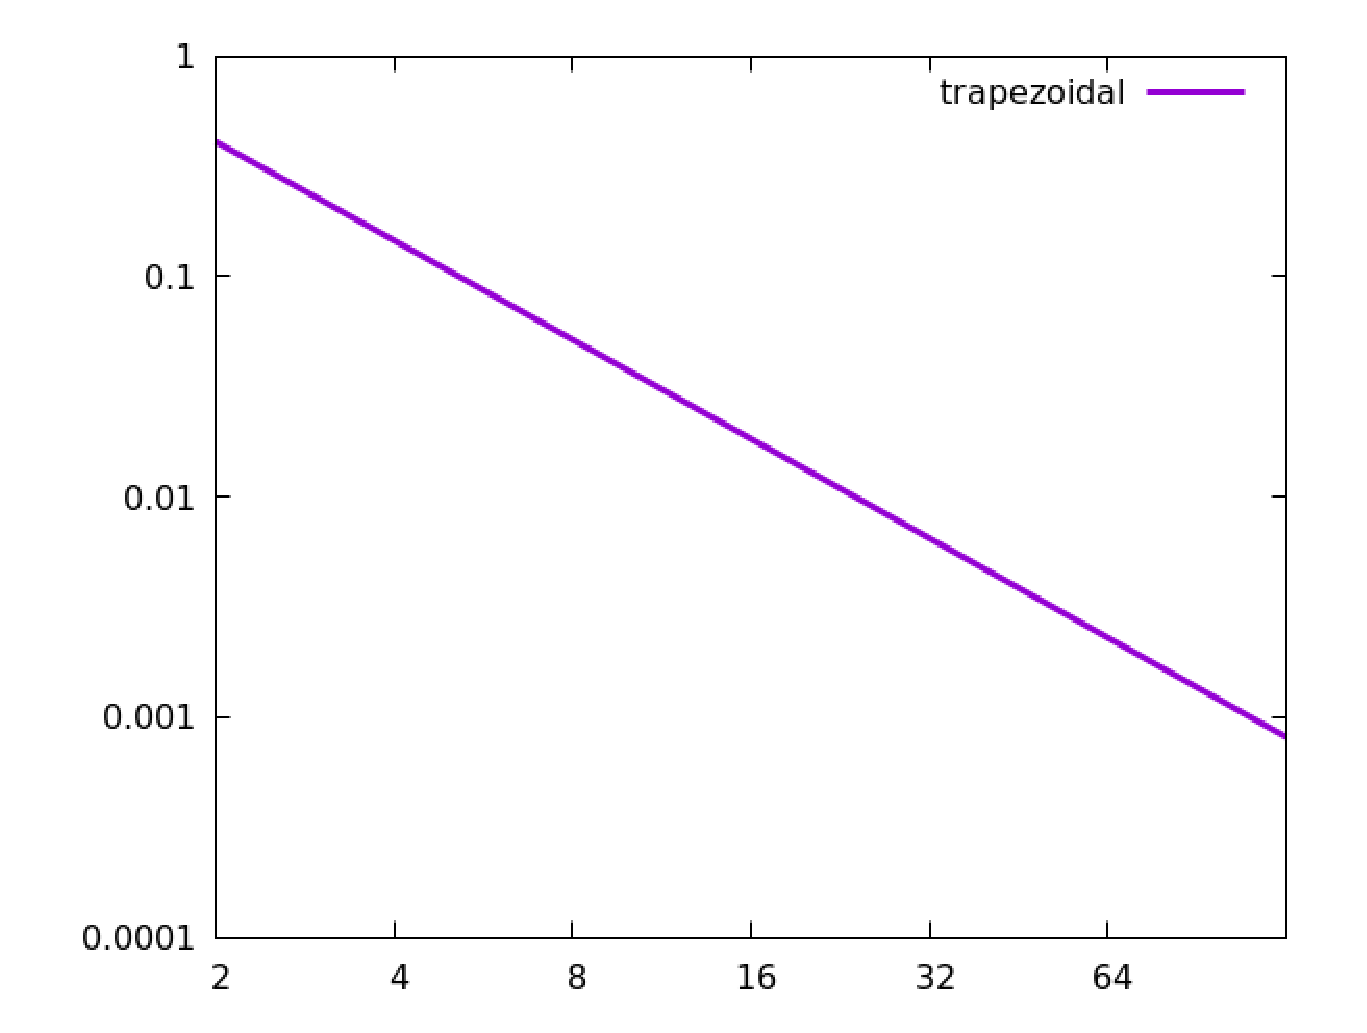
\includegraphics[width=\textwidth]{pictures/tz.eps}
  \caption{台形則による数値解の誤差のグラフ}
  \label{trapezoidal_graph}
\end{figure}

このグラフはx軸が分割数、y軸が真の値と計算値との誤差を表している。
なお、x軸y軸ともに対数が取られていることに注意する。
図\ref{trapezoidal_graph}より、分割数が増えるごとに誤差の値が減少していることがわかる。
具体的には\(\log{x}\)と\(\log{y}\)が負の比例関係で誤差が減少する。
これは台形則での誤差を解析するとわかるが、誤差\(|E|\)が分割の区間\(h\)と定数\(M_1\)、区間の下端と上端\(a, b\)を用いて\(|E| \leq \frac{b-a}{12}M_1h^2\)となることに起因している。
この式は区間の幅が\(\frac{1}{2}\)倍、すなわち分割数が\(2\)倍されると誤差が\(\frac{1}{4}\)倍以下になることを意味している。
故に対数を取れば誤差と分割数の間には負の比例関係があることが示され実際のプログラムの出力にそうような形であることがわかる。


\section*{演習 2: Simpson則による数値積分}

\subsection*{課題 2}

まず、Simpson則による数値計算の誤差をグラフに出力するプログラムを以下に示す。
\begin{lstlisting}[caption={\texttt{Simpson則による数値計算とその誤差を求めるコード}}, numbers=left, label={Simpson1}]
  #include <stdio.h>
  #include <math.h>
  #include <stdlib.h>

  #define A 0.0 // 積分区間の先頭
  #define B 1.0 // 積分区間の最後
  #define N 100 // 分割数

  double func ( double x ) { return 4.0 * sqrt ( 1 - x * x ); }

  double simpson(double (*f)(double), const double a, const double b, const int n) {
      /*
          f: 被積分関数
          a: 下端
          b: 上端
          n: 分割数
      */
      double h = (b - a)/n; // 分割の幅
      double r = 0;

      for(int i = 0; i < n; i += 2) {
          r += h * ((*f)(a + i*h) + 4*(*f)(a + (i+1)*h) + (*f)(a + (i+2)*h)) / 3;
      }

      printf ( "n = %d, r = %1.10f, err = %1.10f\n", n, r, fabs ( r - M_PI ) );

      return fabs(r - M_PI);

  }

  void save_dat(int *x_data, double *y_data, int n) {
    FILE *fout_data = fopen("xy_data.dat", "w");

    for(int i = 0; i < n; i++) {
      int x = x_data[i];
      double y = y_data[i];
      fprintf(fout_data, "%d %lf\n", x, y);
    }
    fclose(fout_data);
  }

  void write_graph(char *file_name) {
    FILE *gp = popen("/usr/bin/gnuplot", "w");
    if(gp == NULL) {
      perror("popne");
      exit(1);
    }

    fprintf(gp, "plot 'xy_data.dat' with line\n");
    fprintf(gp, "set logscale\n");
    fprintf(gp, "set xtics (1, 2, 4, 8, 16, 32, 64, 128)\n");
    fprintf(gp, "set ytics (10, 1, 0, 10**-1, 10**-2, 10**-3, 10**-4, 10**-5, 10**-6, 10**-7, 10**-8)\n");
    fprintf(gp, "plot 'xy_data.dat' with lines lw 3 title 'simpson'\n");


    fprintf(gp, "set terminal pngcairo\n");
    fprintf(gp, "set out'%s'\n", file_name);
    fprintf(gp, "replot\n");

    fprintf(gp, "exit\n");
    fflush(gp);
    pclose(gp);
  }

  int main ( void )
  {
    double a = A, b = B;

    int splits[7] = {2, 4, 8, 16, 32, 64, 128};
    double results[7];

    for(int i = 0; i < 7; i++) {
      results[i] = simpson(func, a, b, splits[i]);
    }

    save_dat(splits, results, 7);

    char *filename = "simpson.png";
    write_graph(filename);

    return 0;
  }

\end{lstlisting}

このプログラムではSimpson則による数値計算をおこなうsimpson関数に加え、プログラム\ref{trapezoidal}と同じようにfunc、save\_dat、write\_graph、main関数がプログラムされている。
simpsonプログラムでは添字の更新を\(+1\)から\(+2\)に変更し、\(i\)番目の小区間の近似面積を小区間の長さを\(h\)として\(\frac{h}{3}(\text{func}(x_i) + 4\text{func}(x_{i+1}) + \text{func}(x_{i+2}))\)と求めている。 \\
\indent 以上のプログラムを実行して得られた分割数と誤差のグラフは以下のようになる。

\begin{figure}[H]
  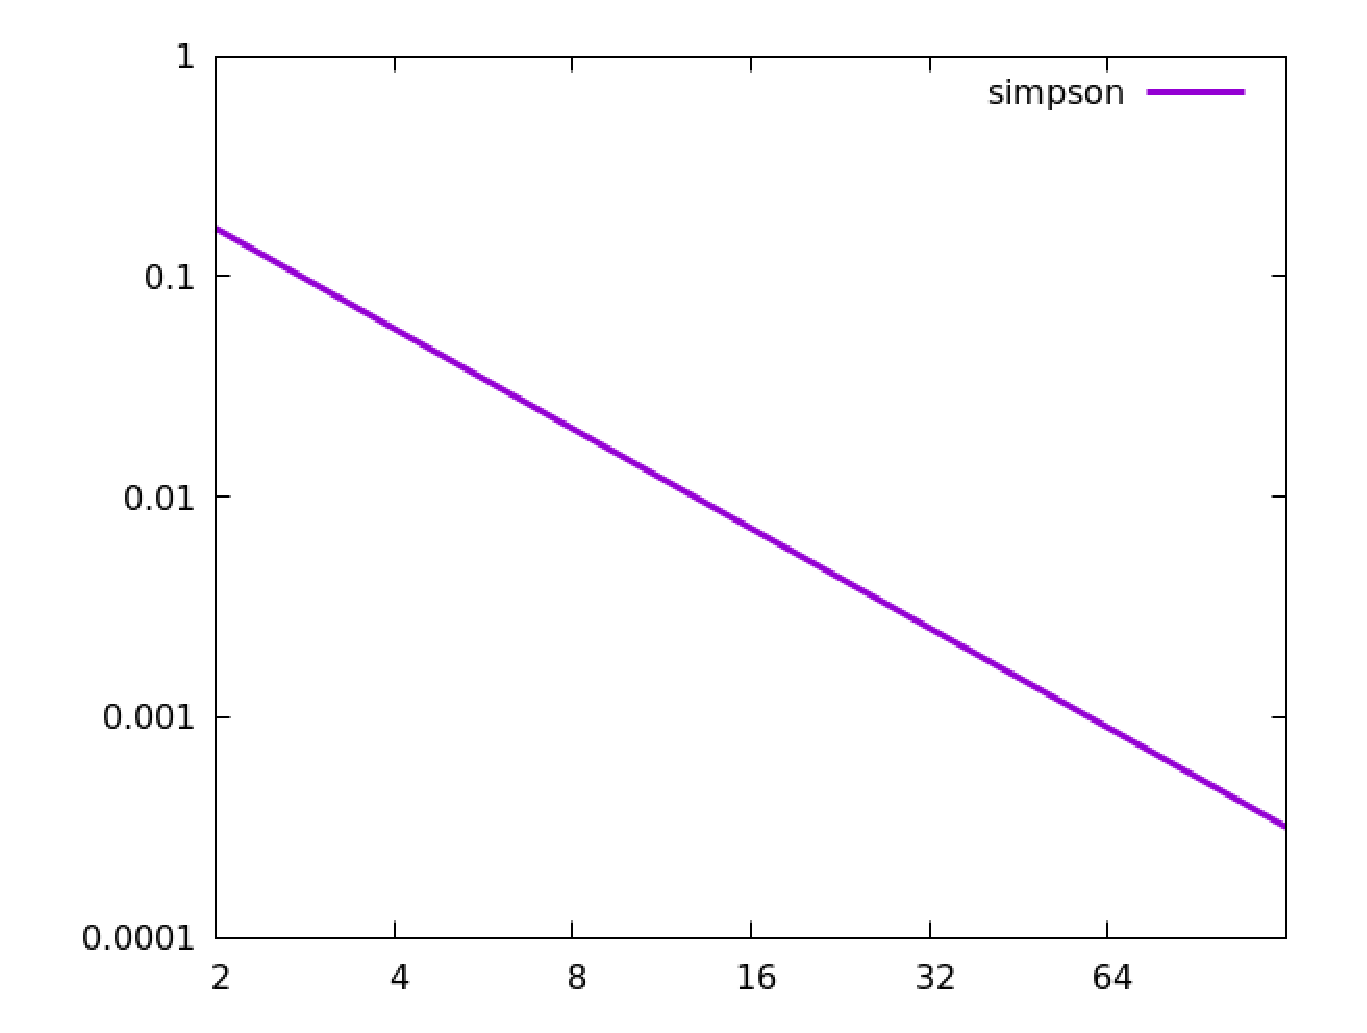
\includegraphics[width=\textwidth]{pictures/simpson.eps}
  \caption{分割数とSimpson則による計算値との誤差のグラフ}
  \label{Simpson_graph_1}
\end{figure}

図\ref{trapezoidal_graph}は図\ref{trapezoidal_graph}と同様に横軸に分割数、縦軸に数値解と真値の誤差を取っており、両軸ともに対数を取ったものとなっている。
図\ref{trapezoidal_graph}と比較すると、図\ref{trapezoidal_graph}と同様に負の比例関係にあるものの、誤差はSimpson則のほうが小さくなっていることがわかる。
これはSimpson則の誤差を解析するとわかる。 \\
\indent Simpson則の誤差\(|E|\)は分割区間を\(h\)、ある定数\(M_3\)を用いて\(|E \leq \frac{b - a}{12}M_3h^4\)と上から抑えることができる。
この結果は分割数が\(2\)倍、すなわち分割区間が\(\frac{1}{2}\)倍されると、誤差は\(\frac{1}{16}\)倍以下になることを示している。
よって、縦軸横軸それぞれ対数を取れば台形則と同様の理由で線形の関係になり、誤差の解析結果から台形則より誤差が小さくなる。
これで、図\ref{Simpson_graph_1}が得られた理由を説明できる。


\subsection*{課題 3}
まず作成したプログラムを載せる。
\begin{lstlisting}[caption={\texttt{変数変換後のSimpson則による分割数と数値解と真値との誤差の}}, numbers=left, label=simpson2]
  #include <stdio.h>
  #include <math.h>
  #include <stdlib.h>

  #define A 0.0 // 積分区間の先頭
  #define B 1.0 // 積分区間の最後
  #define N 100 // 分割数

  double func ( double t ) { return 8.0 * t * t * sqrt(2.0 - t * t); }

  double simpson(double (*f)(double), const double a, const double b, const int n) {
      /*
          f: 被積分関数
          a: 下端
          b: 上端
          n: 分割数
      */
      double h = (b - a)/n; // 分割の幅
      double r = 0;

      for(int i = 0; i < n; i += 2) {
          r += h * ((*f)(a + i*h) + 4*(*f)(a + (i+1)*h) + (*f)(a + (i+2)*h)) / 3;
      }

      printf ( "n = %d, r = %1.10f, err = %1.10f\n", n, r, fabs ( r - M_PI ) );

      return fabs(r - M_PI);

  }

  void save_dat(int *x_data, double *y_data, int n) {
    FILE *fout_data = fopen("xy_data_simpson_2.dat", "w");

    for(int i = 0; i < n; i++) {
      int x = x_data[i];
      double y = y_data[i];
      fprintf(fout_data, "%d %lf\n", x, y);
    }
    fclose(fout_data);
  }

  void write_graph(char *file_name) {
    FILE *gp = popen("/usr/bin/gnuplot", "w");
    if(gp == NULL) {
      perror("popne");
      exit(1);
    }

    fprintf(gp, "plot 'xy_data_simpson_2.dat' with line\n");
    fprintf(gp, "set logscale\n");
    fprintf(gp, "set xtics (1, 2, 4, 8, 16, 32, 64, 128)\n");
    fprintf(gp, "set ytics (10, 1, 0, 10**-1, 10**-2, 10**-3, 10**-4, 10**-5, 10**-6, 10**-7, 10**-8)\n");
    fprintf(gp, "plot 'xy_data_simpson_2.dat' with lines lw 3 title 'simpson2'\n");


    fprintf(gp, "set terminal pngcairo\n");
    fprintf(gp, "set out'%s'\n", file_name);
    fprintf(gp, "replot\n");

    fprintf(gp, "exit\n");
    fflush(gp);
    pclose(gp);
  }

  int main ( void )
  {
    double a = A, b = B;

    int splits[7] = {2, 4, 8, 16, 32, 64, 128};
    double results[7];

    for(int i = 0; i < 7; i++) {
      results[i] = simpson(func, a, b, splits[i]);
    }

    save_dat(splits, results, 7);

    char *filename = "simpson2.png";
    write_graph(filename);

    return 0;
  }

\end{lstlisting}

このプログラムはコード\ref{Simpson1}とほぼ変わらない。唯一変わるのは、func関数が\(t^2\sqrt{2-t^2}\)に対応するように書き換えられている点のみである。
このプログラムを実行すると以下のグラフを得る。
\begin{figure}[H]
  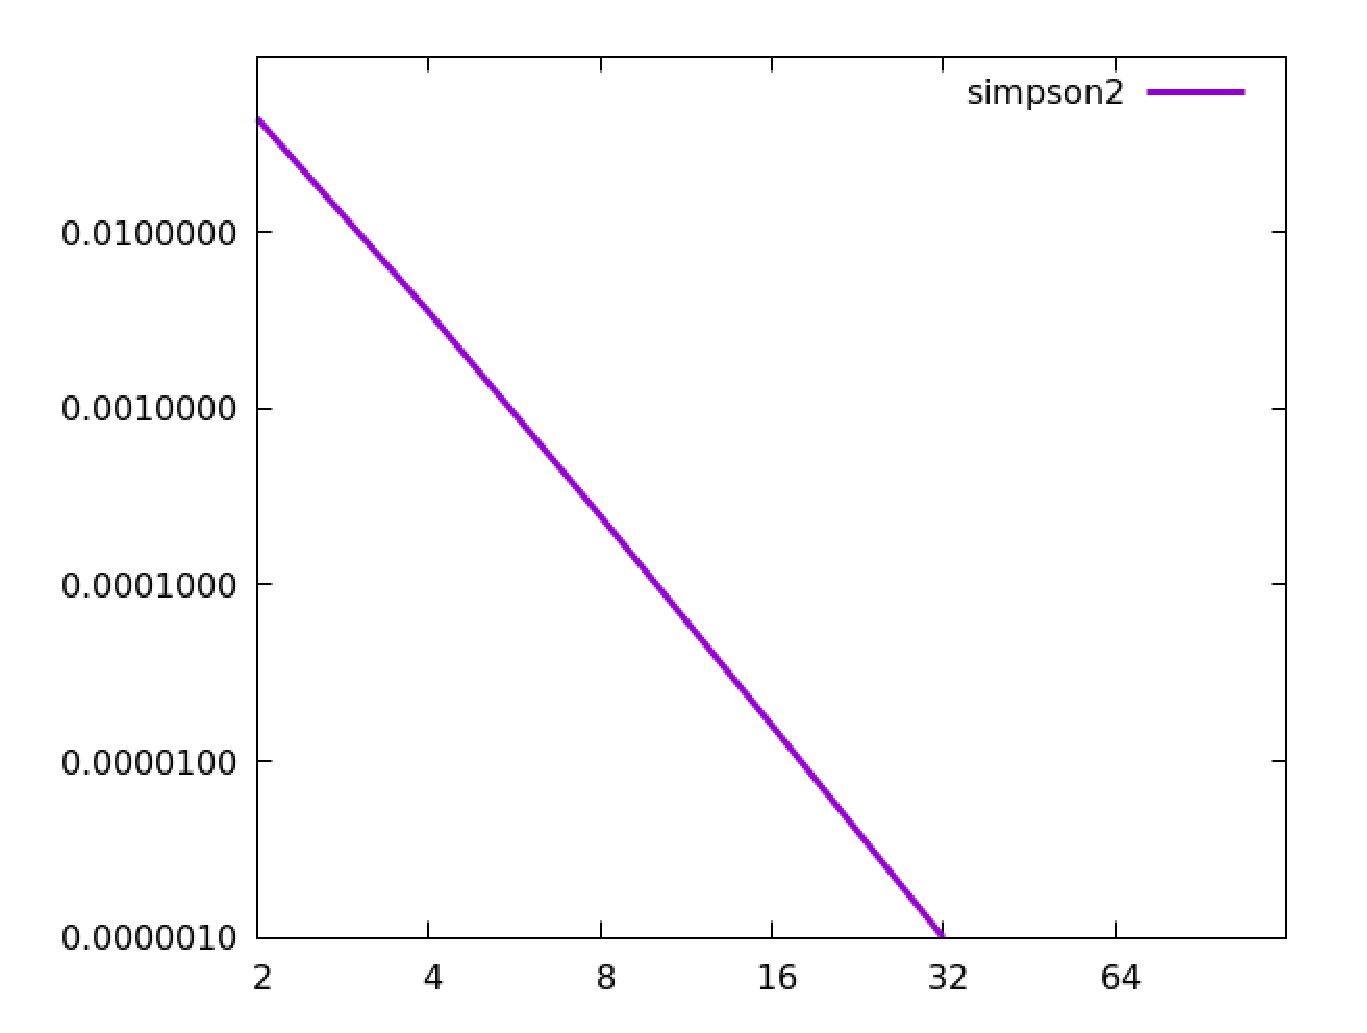
\includegraphics[width=\textwidth]{pictures/simpson2.eps}
  \caption{変数変換後のSimpson則による誤差の数値解析結果}
  \label{simpson_graph_2}
\end{figure}

このグラフの基本的な性質は図\ref{Simpson_graph_1}のときと同じだが、図\ref{Simpson1}と比べて誤差の減少がより早くなっていることがわかる。

\end{document}
